% GigaScience template
\documentclass[a4paper,num-refs]{oup-contemporary}

\journal{gigascience}


%%%% Packages %%%%
\usepackage{siunitx}
\usepackage{minted} % Used for JSON highlighting
\usepackage{algpseudocode} % Algorithmic environment
\usepackage{xspace}
\usepackage{booktabs}

%%%%%%

\usepackage{xcolor}
\usepackage{graphicx}
\usepackage{algorithm}
\usepackage{caption}
\usepackage{subcaption}
\usepackage{listings}
\usepackage{verbatim}
\usepackage{makecell}
\usepackage[flushleft]{threeparttable}

\usepackage{subcaption}
\usepackage{xspace}

%%%% Commands %%%%
\newcommand{\todo}[1]{\color{red}\textbf{TODO:}#1\color{black}}
\newcommand{\note}[2]{\color{blue}Note: #1\color{black}}
\newcommand{\reprozip}[0]{ReproZip\xspace}
\newcommand{\tristan}[1]{\color{blue}\textbf{From Tristan:}#1\color{black}}

 
\title{NURM: a tool to 
locate numerical differences in pipelines}
  
\begin{document}

\author[1]{Ali Salari}
\author[1]{Lalet Scaria}
\author[2,3]{Gregory Kiar}
\author[2]{Lindsay Lewis}
\author[2,3]{Alan C. Evans}
\author[1]{Tristan Glatard}

\affil[1]{Department of Computer Science and Software Engineering, Concordia University, Montreal, Canada}
\affil[2]{McGill University, Montreal, Canada}
\affil[3]{Montreal Neurological Institute, Montreal, Canada}

\maketitle

\begin{abstract} 

Many experiments show that computational analysis results are still not 
completely reproducible. Computational environments including different 
operating systems, hardware categories, and software versions are known 
to have effects on the results produced by analysis pipelines. These 
effects are presumably due to the creation, propagation and 
amplification of small numerical differences across the pipelines. 
Although new techniques such as virtualization, version control 
systems, and provenance management tools provide more reliable 
environment and significantly improve the reproducibility of scientific 
findings. However, the precise causes of such instabilities and the 
path along which they propagate in the pipelines are unclear.  We 
present a technique to identify the processes in the pipeline that 
create numerical differences along the execution, and we apply this 
technique to the HCP structural pre-processing pipelines.

\end{abstract}

\begin{keywords}
Reproducibility; Numerical Instability; Neuroimaging.
\end{keywords}

\section{Introduction}

A reproducible study provides a context in which one is able to get 
results that are consistent with the original 
work~\cite{plesser2018reproducibility}. Research findings are expected 
to be reproducible so that their authenticity and reliability can be 
evaluated. 

Reproducibility is defined as the ability to regenerate the same 
results as the original findings when the experiment is reanalyzed by 
exactly the same analytic methods, software package, parameters, and 
data~\cite{peng2011reproducible}. 

In addition, numerical reproducibility is defined as the ability to 
regenerate bit for bit identical results from multiple 
runs~\cite{hill2017numerical}. This Numerical reproducibility can be 
checked by comparing the binary content of the results which is 
computed by the checksum method.
Regarding these definitions, it must be pointed that a
computation might be reproducible, but not 
be numerically reproducible. For instance, small numerical differences 
created during the pipeline execution may hamper numerical 
reproducibility, but be negligible in the final results.

Recently, scientists began to realize that the results of many 
scientific experiments were not reproducible. According to the previous 
studies, variety of computational infrastructures including workstation 
types, parallelization methods, operating systems, and analysis 
packages are known to influence reproducibility~\cite{Gronenschild2012, 
diethelm2012limits, Glatard2015, bowring2019exploring}.

In particular, the effect of operating system is quantified 
in~\cite{Glatard2015, Gronenschild2012} specially on some of the main 
neuroimaging pipelines including FSL, CIVET and Freesurfer pipelines. 
The binary differences are measured by the checksum method between 
results of the same analyses on different operating systems, which 
indicate a significant disparity. 

This irreproducibility issues are reported as the result of the 
creation, propagation, and amplification of small numerical 
differences~\cite{Gronenschild2012, diethelm2012limits, Glatard2015, 
bowring2019exploring}. In this case, the analysis pipelines are said to 
be numerically unstable. Numerical instability is a characteristic of 
the pipelines which amplify small numerical differences and then hamper 
the reproducibility of the analyses depending on the length of the 
pipeline and magnitude of the differences. In many cases, numerical 
instability is an important issue for reproducibility.

There are different solutions to make reproducible analysis including 
containerization techniques that encapsulate software/hardware 
dependencies, provenance capturing tools, and version control systems. 
However, a comprehensive solution requires to fix the numerical 
instabilities. For this purpose, we introduce a Numerical 
Reproducibility Measurement (NURM) tool to identify the processes in 
pipeline that create numerical differences across several runs. In this 
paper, the execution results of pipelines across different operating 
systems are considered to find out the cause of the irreproducibility 
using the interposition techniques.

The remainder of this paper describes the NURM-tool in different parts 
including the way of capturing and representation of the provenance 
information, the method of clustering of different subject types, and 
process classification to characterize differences. We describe the HCP 
preprocessing pipelines as a popular neuroimaging project to test the 
NURM-tool and evaluate its functionality. Finally, we reported the 
experimental results which describe the processes that are responsible 
for the differences in the pipelines.


\section{Tool description}

Figure~\ref{fig:overview} shows an overview of our method.
For each tested condition, the
pipeline is containerized using Docker, and its interface is
described using Boutiques~\cite{glatard2017boutiques}. \reprozip
is added to the container images for provenance tracking. Our tool first
clusters the subjects based on the similarity of their process trees
produced by \reprozip (Fig.~\ref{fig:overview-cluster}). This results in a
reduced set of representative process trees to evaluate. The processes in
each representative process tree are labeled \tristan{Replace
``classification'' by ``labelling'' everyrwhere} from potential differences
found in their outputs produced in the tested conditions (Fig.~\ref{fig:overview-classify}).
To do that, a difference file is first produced that contains all the
files with differences across conditions
(Fig.~\ref{fig:overview-classify} - (A)\tristan{Add labels to the figure}).
Differences are identified simply by comparing file checksums. Using the
difference file, we then classify processes in 4 categories (Fig.~\ref{fig:overview-classify} - (B)) depending
whether they create differences (represented in red), remove differences
(blue), neither create nor remove differences (green), or have uncertain
behavior (yellow). When processes with an uncertain behavior are found, the
pipeline in condition 2 is modified (as explained later) and re-executed. This
procedure iterates until all processes are classified. 
\begin{figure}
  \centering
  \begin{subfigure}{\columnwidth}
    \centering
    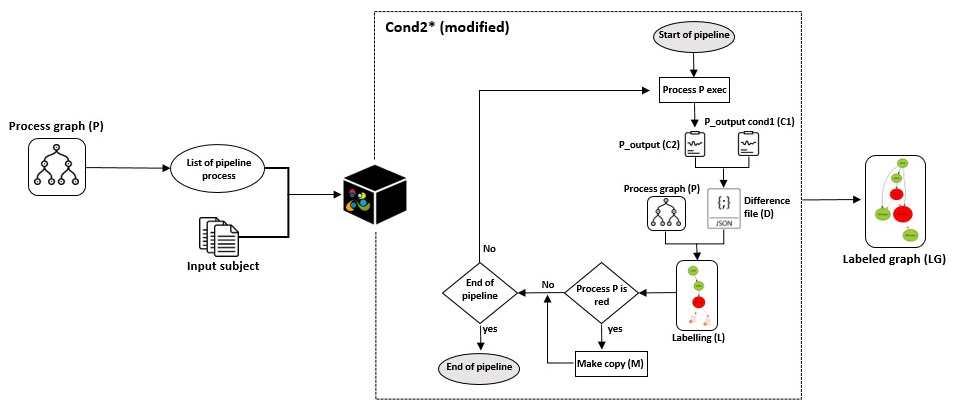
\includegraphics[width=.7\columnwidth]{images/Slide1}
    \caption{Subject clustering.}
    \label{fig:overview-cluster}
  \end{subfigure}
   \begin{subfigure}{\columnwidth}
    \centering
     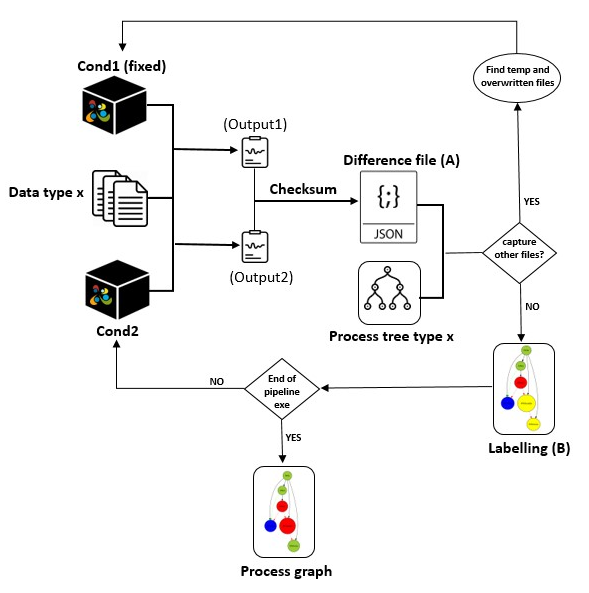
\includegraphics[width=.75\columnwidth]{images/Slide2}
     \caption{Process classification.}
     \label{fig:overview-classify}
   \end{subfigure}
   \caption{Method overview}
   \label{fig:overview}
  \end{figure}

\subsection{Provenance capture and representation}

We use the \reprozip tool~\cite{Chirigati2016} to record: (1) 
the tree of processes executed by the pipeline and (2) the list of 
files read and written by each process. This information is collected 
by system call interceptions, through the \texttt{ptrace} Unix system 
call, and stored in a \texttt{SQLite} database. The database stores 
information of all the processes which are created by the 
\texttt{clone()} or \texttt{fork()} system calls. It also records the 
files opened by each process (in read, write or execution mode), 
including the result files and the temporary files.

NURM-tool reconstructs the tree of processes starting from the first 
process created by the pipeline and through identifying its child 
processes as the ones that were created through \texttt{clone()} or 
\texttt{fork()}. It creates a process graph from this tree by adding 
edges corresponding to file dependencies between processes. A file 
dependency is defined between processes A and B if a file written by A 
is read by B. Figure~\ref{fig:simple_script} shows an example of a 
process tree constructed for the simple bash script illustrated in 
Algorithm~\ref{algo:sample-script} from the brain extraction procedure.


\begin{algorithm}[h!]
\caption{Sample script from brain extraction process}
\label{algo:sample-script}
\begin{verbatim}
#!/bin/bash
if [ # !=1 ]
then
    echo "usage: 0 <inputimage.nii.gz>"
    exit 1
fi
input_image=$1
bet_output="$(basename ${input_image} 
                       .nii.gz)_brain.nii.gz"
bet_output_binarized="$(basename ${input_image} 
                       .nii.gz)_brain_bin.nii.gz"

bet ${input_image} ${bet_output} > bet_temp.out
echo "Voxels / Volume in brain mask:"
fslstats ${bet_output} -V
fslmaths ${bet_output} ${bet_output_binarized}
echo "Voxels / Volum in binarized brain mask:"
\rm bet_temp.out
\end{verbatim}
\end{algorithm}

\begin{figure}
\centering
  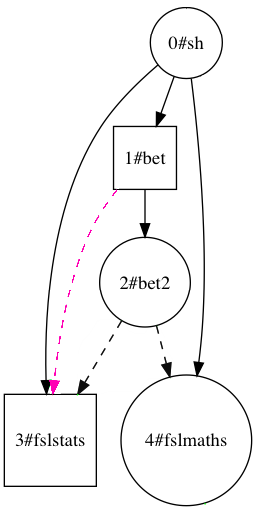
\includegraphics[scale=0.25]{images/simple_graph}
  \caption{Process tree constructed from an example brain extraction
	script. Every node in the graph is labeled using (1) a process id 
	created by our reconstruction, (2) the name of the executable run 
	by the process. Processes that read or write temporary files are 
	represented with squares; other ones with circles. Plain edges 
	represent the process tree (\texttt{fork()} or \texttt{clone()} 
	system calls). Dashed edges represent file dependencies: temporary 
	files are in yellow and result files are in green.}
  \label{fig:simple_script}
\end{figure}

\subsection{Subject type}

Depending on the variety of computing environments, in particular, 
different analysis software packages, different process trees can be 
constructed for the same experiment. It was expected to achieve the 
same process trees since we used the same computing environments 
specially the same analysis software package in different conditions. 
However, we found that different subjects may result in different 
process trees. 

Therefore, all subjects should be grouped into different types based on 
the topological structure of the process trees.
To this order, the distance between trees, topological differences, 
need to be calculated.

We used the tree edit distance~\cite{zhang1989simple} method to measure 
the distance between labeled trees. The distance between two labeled 
trees is defined as the minimum weighted number of edit operations that 
it takes to transform one tree to another. There are three edit 
operations that can be used to transform a tree including modify, 
remove, and insert. Modifying node \textit{n} means changing the label 
on \textit{n}. Removing node \textit{n} means making the children of 
\textit{n} become the children of its parent and then 
deleting it. Inserting is the complement of remove; this 
means that inserting \textit{n} as the child of \textit{n}$'$ will make 
\textit{n} the parent of a consecutive subsequence of the current 
children of \textit{n}$'$.
Each operation has an associated cost---insertions and removals each 
cost 1, and modifications cost either 1 or 2, depending on whether 
you consider a modification to essentially be just a removal 
or followed by an insertion.

We clustered subjects into various types using the bottom-up hierarchical 
clustering approach implemented in \textit{scipy} python package (see 
Algorithm~\ref{algo:hclustering}). This approach groups together the 
subjects with similar distance, less than a threshold. 

% \texttt{agglomerative approach}
%  based on \texttt{nearest\_neighbors} method
  
\begin{algorithm}[h!]
\caption{Hierarchical clustering algorithm from \textit{scipy}}
\label{algo:hclustering}
\begin{algorithmic}

  \State /* Input: a list of n trees; \texttt{T = [t${_1}$, t${_2}$,...,t${_n}$]}
  \State /* Output: a list of clusters; \texttt{C = [c${_1}$,c${_2}$,...,c${_k}$]}
  \For{\texttt{i=1} in \texttt{n}}
  \State \texttt{C${_i}$} = \texttt{T${_i}$} 
  \State \texttt{\# Create a cluster for each tree in input list;}
  \EndFor
  \While{\texttt{len(C)} > \texttt{1}}  
  \For{\texttt{i=1} to \texttt{n}}
  \For{\texttt{j=i+1} to \texttt{n}}
  \State \texttt{D${_{ij}}$} = \texttt{edit\_distance(C${_i}$, C${_j}$)}
  \State \texttt{\# Select two nearest clusters;}
  \EndFor
  \EndFor
  \State \texttt{d\_min${_{ij}}$} = \texttt{MIN(D)}
  \If{\texttt{d\_min${_{ij}}$} > \texttt{thre}}
  \State Return \texttt{C}
  \Else {
  \State \texttt{C${_i}$} = Merge(\texttt{C${_i}$ and C${_j}$})
  \State Remove \texttt{C${_j}$}}
  \EndIf
  \EndWhile
%  \State Function edit\_distance (C${_1}$, C${_2}$)
%  \State EndFunction
\end{algorithmic}
\end{algorithm}

The clustering algorithm starts by finding two closest subjects to each 
other on the basis of edit distance method and form a new cluster 
between them. In the next iteration, this cluster aggregates with the 
next nearest cluster or subject and turns to another cluster. This 
process continues until all the subjects are aggregated to form one big 
cluster or the distances are less than an specified threshold. The 
threshold is defined as the minimum distance required to separate 
clusters. 


\subsection{Tree analysis}

NURM-tool classifies the processes into four 
categories based on the process tree and the \textit{difference} JSON file 
mentioned in the previous sections:
\begin{enumerate}
\item Processes that read and write files that do not have differences 
are \emph{transparent} (Figure~\ref{fig:processes}.a).
\item Processes that read files 
that do not have any differences but write files that have differences 
\emph{create} differences in the pipeline (Figure~\ref{fig:processes}.b).
\item Processes that read files 
that have differences and write files that do not have differences \emph{remove} 
differences from the pipeline (Figure~\ref{fig:processes}.c).
\item Processes that read files that have differences and write files that 
also have differences are 
\emph{unknown} (Figure~\ref{fig:processes}.d).
\end{enumerate}

\begin{figure}%\centering
\centering
    \begin{subfigure}{0.4\linewidth}
        
\includegraphics[scale=0.34]{images/green.png}
        \caption{Transparent}
        \label{fig:green}
    \end{subfigure}
    \hfill
    \begin{subfigure}{0.4\linewidth}
    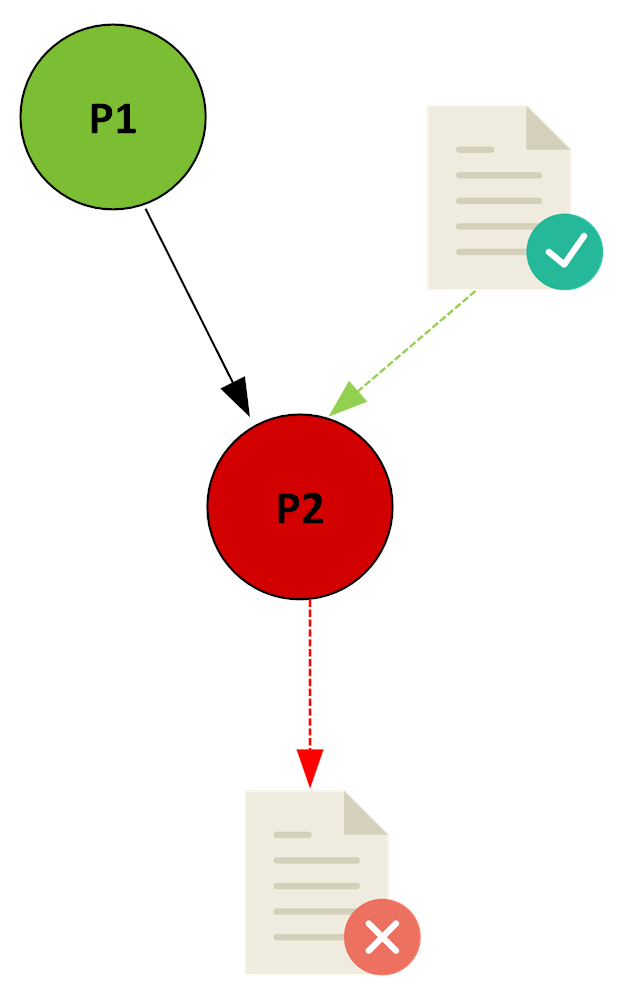
\includegraphics[scale=0.34]{images/red.png}
    \caption{Creates differences}
    \label{fig:red}
    \end{subfigure}
    \hfill
    \begin{subfigure}{0.4\linewidth}
    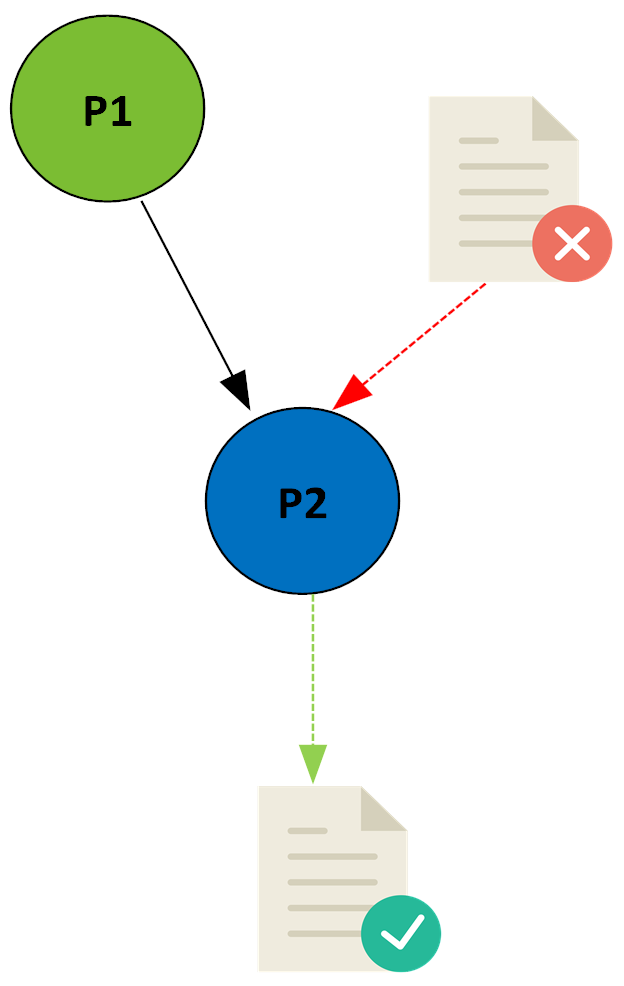
\includegraphics[scale=0.34]{images/blue.png}
    \caption{Removes differences}
    \label{fig:blue}
    \end{subfigure}
    \hfill
    \begin{subfigure}{0.4\linewidth}
    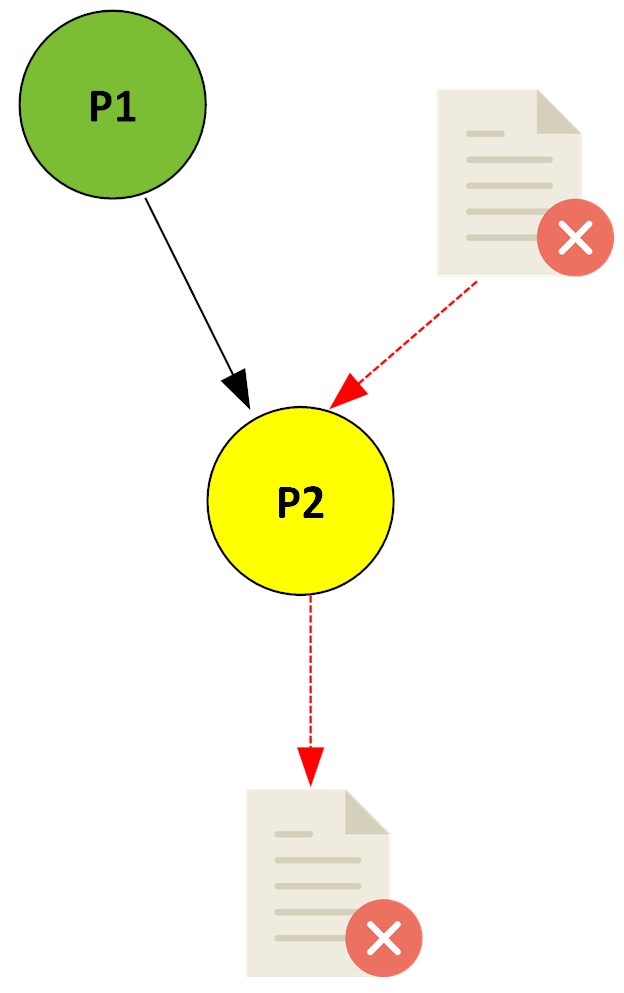
\includegraphics[scale=0.34]{images/yellow.png}
    \caption{Unknown}
    \label{fig:yellow}
\end{subfigure}
    \caption{Different type of classified process based on the input/output files.
  Dashed edges refer to the file dependencies between processes A and B 
  if a file written by A is read by B. Solid black edges refer to the 
  relationship between parent and child processes.}
    \label{fig:processes}
\end{figure}

There are some issues that should be addressed to classify process 
properly, including capturing temporary files that have been removed 
during the execution, capturing files written by multiple processes, 
and unknown process.

\subsubsection{Capture temporary files} 
The classification of processes that read or 
write temporary files is uncertain when these files are deleted during 
the execution. To address this issue, we replace every process P that 
writes temporary files with a modification of P that first calls P and 
then backs up all its output files to a read-only directory. This 
replacement is done by modifying the Unix PATH variable to point to a 
directory containing the modified versions of the processes. This 
solution does not cover the temporary files that are removed by P 
itself; this is not a problem since these files do not play any role in 
the subsequent steps of the pipeline, by definition. 

\subsubsection{Capture multiple write files} 
Files written by multiple processes also lead 
to unknown classification labels. To address this issue for a file F 
written by processes in \textbf{P} = \{$P_{1}$, \ldots $P_{n}$\}, we 
(1) check that processes in \textbf{P} do not write concurrently to F, 
(2) we establish an order on \textbf{P} based on the creation timestamp 
of the processes, (3) we replace ever process $P_{i}$ in \textbf{P} by 
a wrapper that first calls $P_{i}$ and then backs up F to a read-only 
directory. Thus, multiple versions of F are saved and used in the 
analysis. 

Furthermore, cycles may be present in the process tree in case a file 
was written by more than one process. We remove such cycles by removing 
file edges between processes A and B when A's process creation 
timestamp is posterior to B's or when A=B. Indeed, such edges cannot 
happen in practice unless A and B were running concurrently, which we 
assume is not the case (we also checked that on the workflow we 
tested). 

\subsubsection{Unknown process} 
Another challenge is to classify processes that 
read files that have differences and write files that also have differences. In 
such situations, it is not possible to determine from the pipeline 
results whether the process created differences, removed some differences, or was 
transparent. We label such processes \emph{unknown}.
To address this issue, we developed an iterative approach that 
consists of the following steps: 

\begin{enumerate}
  \item Run the pipeline in conditions 1 and 2; classify the
    processes as \emph{transparent}, \emph{create differences},
    \emph{remove differences} or \emph{unknown}.
  \item If there are \emph{unknown} processes then: replace each 
  process P that create differences by a process Q that copies the results 
  produced by process P in condition 1 to the pipeline output in 
  condition 2. 
  \item Repeat steps 1 and 2 until there is no \emph{unknown} process left.
\end{enumerate}

The replacement of process P at step 2 is done by replacing P with a 
custom script produced by step 1. This custom script copies the results 
obtained in condition 1 if it is invoked with the arguments of a 
process that created differences, and calls P's original executable 
otherwise. The replacement is done through the PATH variable, as 
before. This algorithm converges to a process tree without any 
\emph{unknown} process after a finite number of iterations.

\begin{figure}
  \centering
  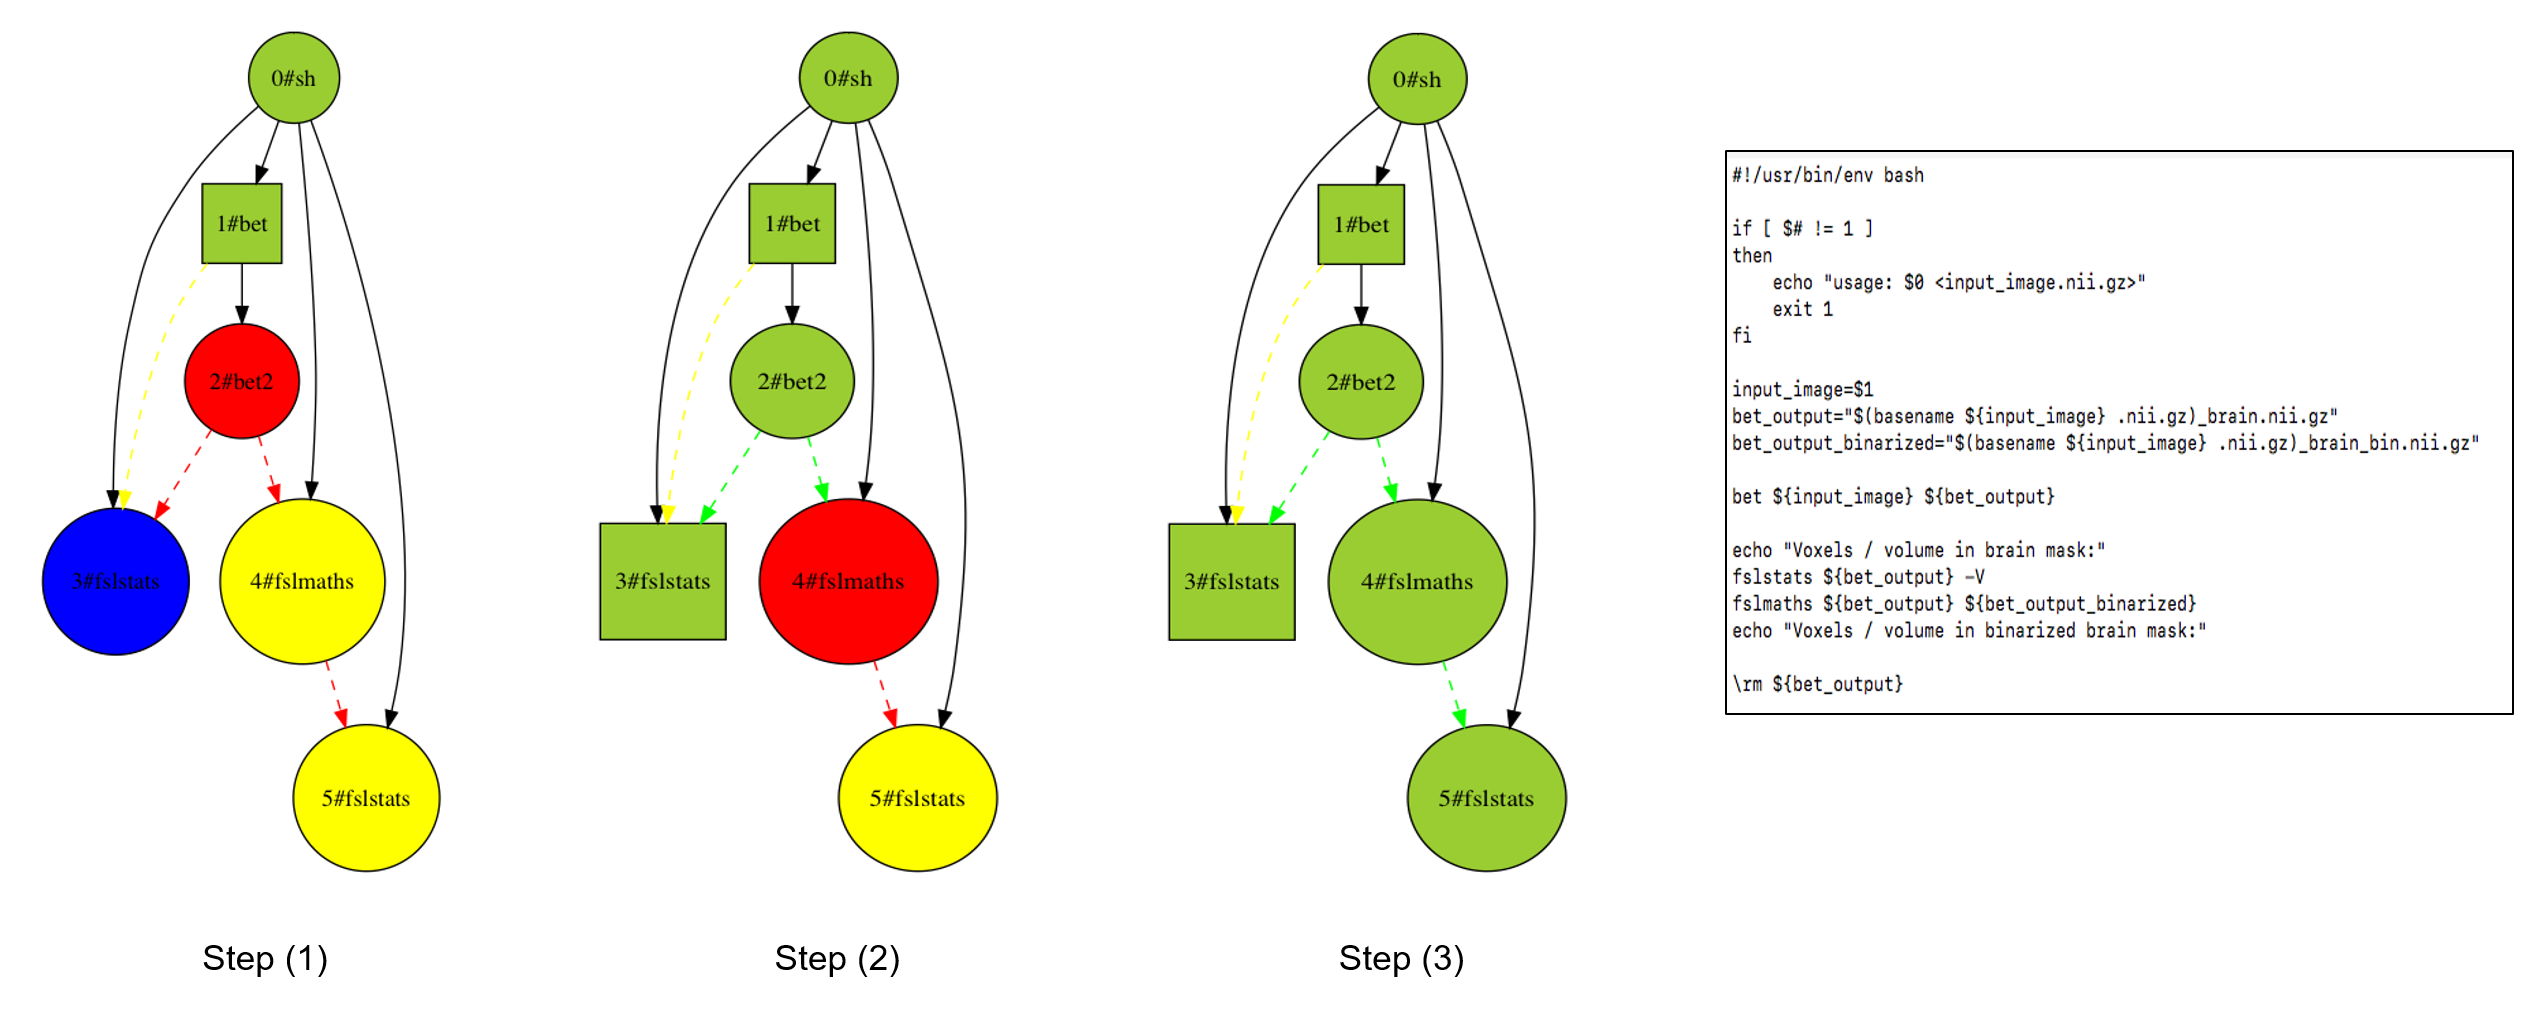
\includegraphics[width=\columnwidth]{images/iterative_modif}
  \caption{iteration of proposed modification.}
  \label{fig:iterations}
\end{figure}

Figure~\ref{fig:iterations} illustrates our iterative classification 
process for the example in Figure~\ref{fig:simple_script}. At every 
step, processes that created differences are shown in red, processes that 
removed differences are in blue, processes that propagated differences are in 
yellow, and other processes (transparent processes) are in green. As in 
Figure~\ref{fig:simple_script}, plain black edges represent the process 
tree and dashed edges represent file dependencies: green edges 
represent files with no differences, while red edges represent files with 
differences. Temporary files are not represented because they have been 
backed up as previously described.

The three steps in Figure~\ref{fig:iterations} correspond to the 
iterations of the classification algorithm. At step one, \texttt{2\#bet2} 
is classified as difference creator (red) as it produced files with differences 
from files without differences. \texttt{3\#fslstats} is classified as difference  
remover (blue) as it produced files without differences from files with 
differences. \texttt{4\#fslmaths} and \texttt{5\#fslstats} are classified as 
unknown (yellow) as they produce files with differences from files with 
differences.

At step 2, the files produced by \texttt{2\#bet2} in the tested 
condition are replaced with the files produced by \texttt{2\#bet2} in 
the other condition. \texttt{3\#fslstats} is now classified as 
transparent, \texttt{4\#fslmaths} is now classified as difference creator 
and \texttt{5\#fslstats} is still unknown.

At step 3, the files produced by \texttt{4\#fslmaths} in the tested 
condition are replaced with the files produced by \texttt{4\#fslmaths} 
in the other condition. \texttt{5\#fslstats} is now transparent.
 
As a result of those 3 steps, the final process classification is: 
\texttt{2\#bet2} and \texttt{4\#fslmath} are difference creators (red), 
\texttt{3\#fslstats} is difference remover (blue) and the other processes 
are transparent.


\section{Experiments}

\subsection{HCP pipelines and datasets}

The Human Connectome Project (HCP)~\cite{glasser2013minimal} developed 
a set of pipelines to help extraction of structural, functional or 
diffusion MRI data across a large set of high resolution MR images. 
These pre-processing pipelines create results that are available in 
standard volume and combined surface and volume spaces which makes it 
easier for researchers to compare the images across the neuroimaging 
spectrum. 

We focused on HCP structural pre-processing pipelines to (1)quantify 
the effect of OS on HCP pre-processing pipelines (2) identify the 
process(es) in the pipelines that are responsible for such effects.

The structural pre-processing pipelines consists of PreFreeSurfer, 
FreeSurfer and PostFreeSurfer. In this paper, 
we analyzed PreFreeSurfer pipeline which consist of various steps 
including correction of MR 
gradient nonlinearity distortions, align the T1w and T2w images using 
FSL FLIRT, Align native space to MNI template using ACPC and FSL FLIRT, 
brain extraction usin FSL FLIRT and FNIRT to MNI template, register T2w 
to T1w using FLIRT's BBR, perform a bias field correction, and register 
the subject's native structural space to MNI space.  

We randomly selected 100 subjects from the HCP data release S500 and then 
using the NURM-tool we cluster them into different groups. 
Figure~\ref{fig:subj-clusters} shows the result of data clustering. 
Among our dataset, we identified 4 types of subjects with 
different topology of process trees. In addition, we verified that 
the process trees were identical for all subjects of the same type in 
different versions of CentOS operating system. The remainder of the 
analysis is done separately for each subject type.

%\begin{figure}
%\centering
%  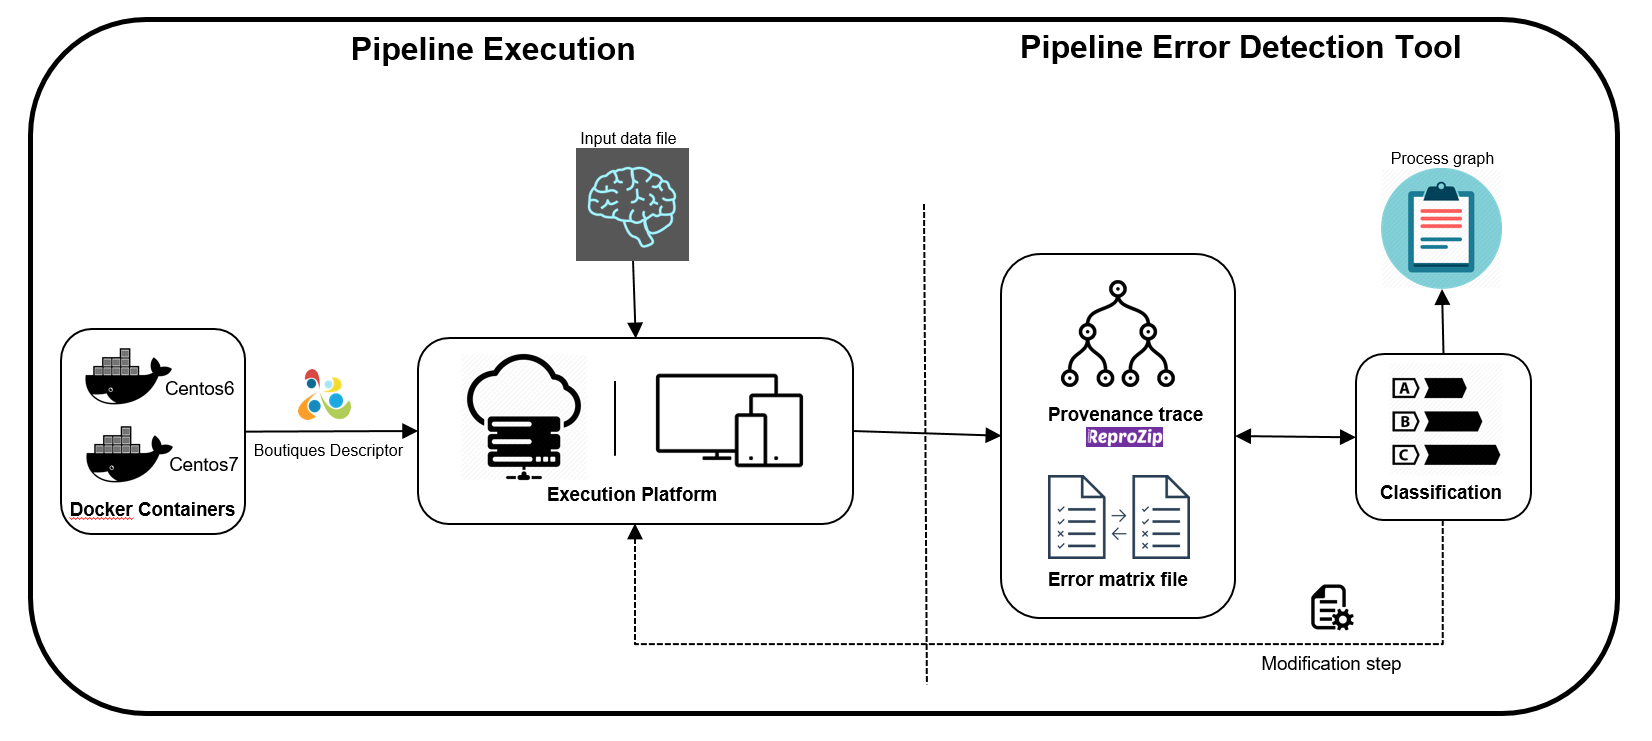
\includegraphics[width=\columnwidth]{images/overview.png}
%  \caption{An overview of the proposed technique.}
%  \label{fig:overview}
%\end{figure}


%\begin{table}
%\centering
%\begin{threeparttable}
%\caption{An overview of the HCP data (Humman Connectome DB).}
%
%\begin{tabular}{@{}llllll@{}}
%\toprule
%Subject & Release & Acquisition & Gender & Age      & Subj\_Type   \\ \midrule
%103515  & Q1      & Q02         & F      & 26-30    & type1         \\
%105216  & Q3      & Q03         & M      & 26-30    & type4         \\
%103414  & Q2      & Q02         & F      & 22-25    & type1         \\
%125525  & Q1      & Q01         & F      & 31-35    & type1         \\
%142828  & Q1      & Q01         & M      & 31-35    & type1         \\
%129533  & Q3      & Q04         & F      & 31-35    & type1         \\
%103818  & Q1      & Q01         & F      & 31-35    & type3         \\
%133928  & Q2      & Q03         & M      & 26-30    & type3         \\
%148032  & Q3      & Q03         & F      & 31-35    & type2         \\
%139637  & Q2      & Q03         & F      & 31-35    & type1         \\ \bottomrule
%\end{tabular}
%\begin{tablenotes}
%      \small
%      \item *Subj\_Type refers to the tree topology type of the subjects.
%\end{tablenotes}
%\end{threeparttable}
%\label{table:data}
%\end{table}



\subsection{Results}

We executed the pipelines using Docker containers to simplify the 
deployment of different operating system versions on execution 
platforms. The Docker images were built for the HCP PreFreeSurfer 
pipeline v3.19.0 in 
CentOS 6.8 and CentOS 7.2. Docker images are available on DockerHub for 
reuse \url{https://hub.docker.com/r/bigdatalabteam/hcp-prefreesurfer/}. 
We collected the provenance trace (tree of executed processes and files 
accessed in read or write mode) for each type of 
subjects(Table~\ref{table:data}) using system-call interception as 
provided by the \reprozip tool~\cite{Chirigati2016}.

Two types of errors can occur in the subjects due to the 
errors in the operating systems. One is inter-OS error caused by the 
operating system library updates and the other type, intra-OS errors 
occurs as a result of the pseudo-random processes used in the 
pipelines. An example of a pseudo-random process function is, a random 
number generator that would get initialized using a seed state. the 
proposed method can be used to identify both kind of errors. The files 
that are common to all the subjects only are taken into consideration 
for comparison. The first step is identification of files with 
differences in their checksums. This is identified using the checksums 
that are recorded after the processing. Intra-OS errors are identified 
using the run-number added as the suffix for the conditions. For 
example, the two batches of subjects processed under the same condition 
(CentOS6) are stored as run-1 and run-2. The files belonging to the 
subjects stored under the above mentioned conditions are treated as 
intra-OS runs.


\subsubsection{Inter-OS binary differences}


In the previous study~\cite{Scaria2017}, we showed that pre-processing 
pipelines of the Human Connectome Project~\cite{Glasser2013} were 
sensitive to operating system variation so that Figure 
\ref{fig:tissue_class} illustrates the binarized errors after brain 
tissue segmentation process in FreeSurfer. In addition, 
Figure~\ref{fig:fnirt_result} shows the same errors occurred in 
non-linear registration process between CentOS6 and CentOS7 in PreFreeSurfer. 

\begin{figure}
%  \includegraphics{brain\_classification}
\centering
  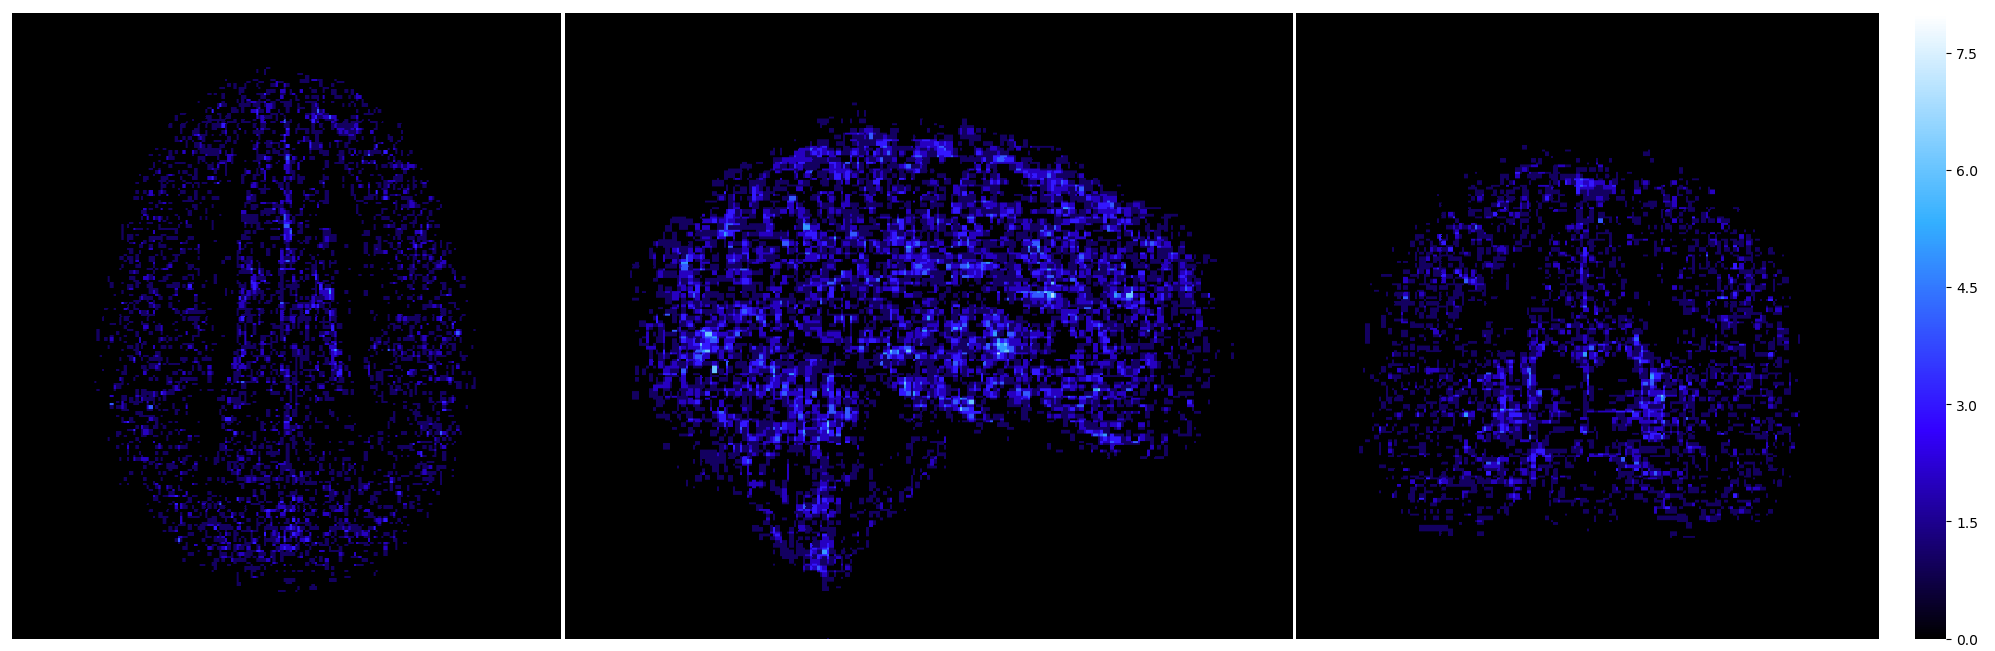
\includegraphics[width=\columnwidth]{images/brain_classification.png} 
  \caption{Binarized error between brain segmentation results from 
  FreeSurfer, subject 105216 (CentOS6 vs. CentOS7)~\cite{Scaria2017}.
    } 
  \label{fig:tissue_class}
\end{figure}

\begin{figure}
\centering
  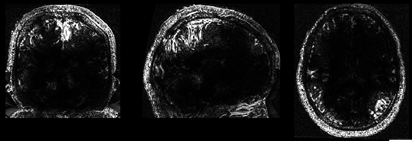
\includegraphics[width=\columnwidth]{images/fnirt_result.png} 
  \caption{Absolute errors between FNIRT results from PreFreeSurfer 
  (T2w\_acpc\_to\_MNI\_nonli.nii.gz), subject 104820 (CentOS6 vs. 
  CentOS7)~\cite{Scaria2017}. } 
  \label{fig:fnirt_result}
\end{figure}

\subsubsection{PreFreeSurfer pipeline analysis} 

We identified processes that introduce errors in PreFreeSurfer 
pipeline. Among the 117 data files produced by PreFreeSurfer, 21 did 
not have any error for any subject, 92 had errors for all subjects and 
4 had errors for 3 subjects only. 

Figure \ref{fig:complete-graph} shows the annotated provenance graph 
of the PreFreeSurfer pipeline executed on CentOS6 and CentOS7. Each 
node in the graph represent an executed process in the pipeline. 
Processes that created errors are shown in red, processes that removed 
errors are in blue, and other processes are in green.  Squares denote 
processes for which the classification is uncertain, due to temporary 
files that were removed during the execution. Black edges link 
sub-processes to their parents while dashed edges denote file 
dependencies between processes (green edges: files with no errors; red 
edges: files with errors; yellow edges: temporary files).

The processes that introduce errors in PreFreeSurfer along with the 
number of occurrences are depicted in Figures~\ref{fig:pfs_table, 
fig:pfs_chart} including linear registration with “\emph{FLIRT}” (in 
ACPC Alignment, BrainExtraction, DistortionCorrection, 
AtlasRegistration), non-linear registration with “\emph{FNIRT}” (in 
BrainExtraction and AltasRegistration), image warping with 
“\emph{new\_invwarp}” (in BrainExtraction and AtlasRegistration).  In 
addition, errors were observed in image mean and standard-deviation 
computations with “\emph{fslstats}” (in BiasFieldCorrection), and in 
masked image extrapolation with “\emph{fslmaths}” (in 
BiasFieldCorrection).  Besides, transformation format conversion with 
“\emph{convertwarp}” (in DistortionCorrection) was able to remove 
errors.

\begin{figure}
\centering
  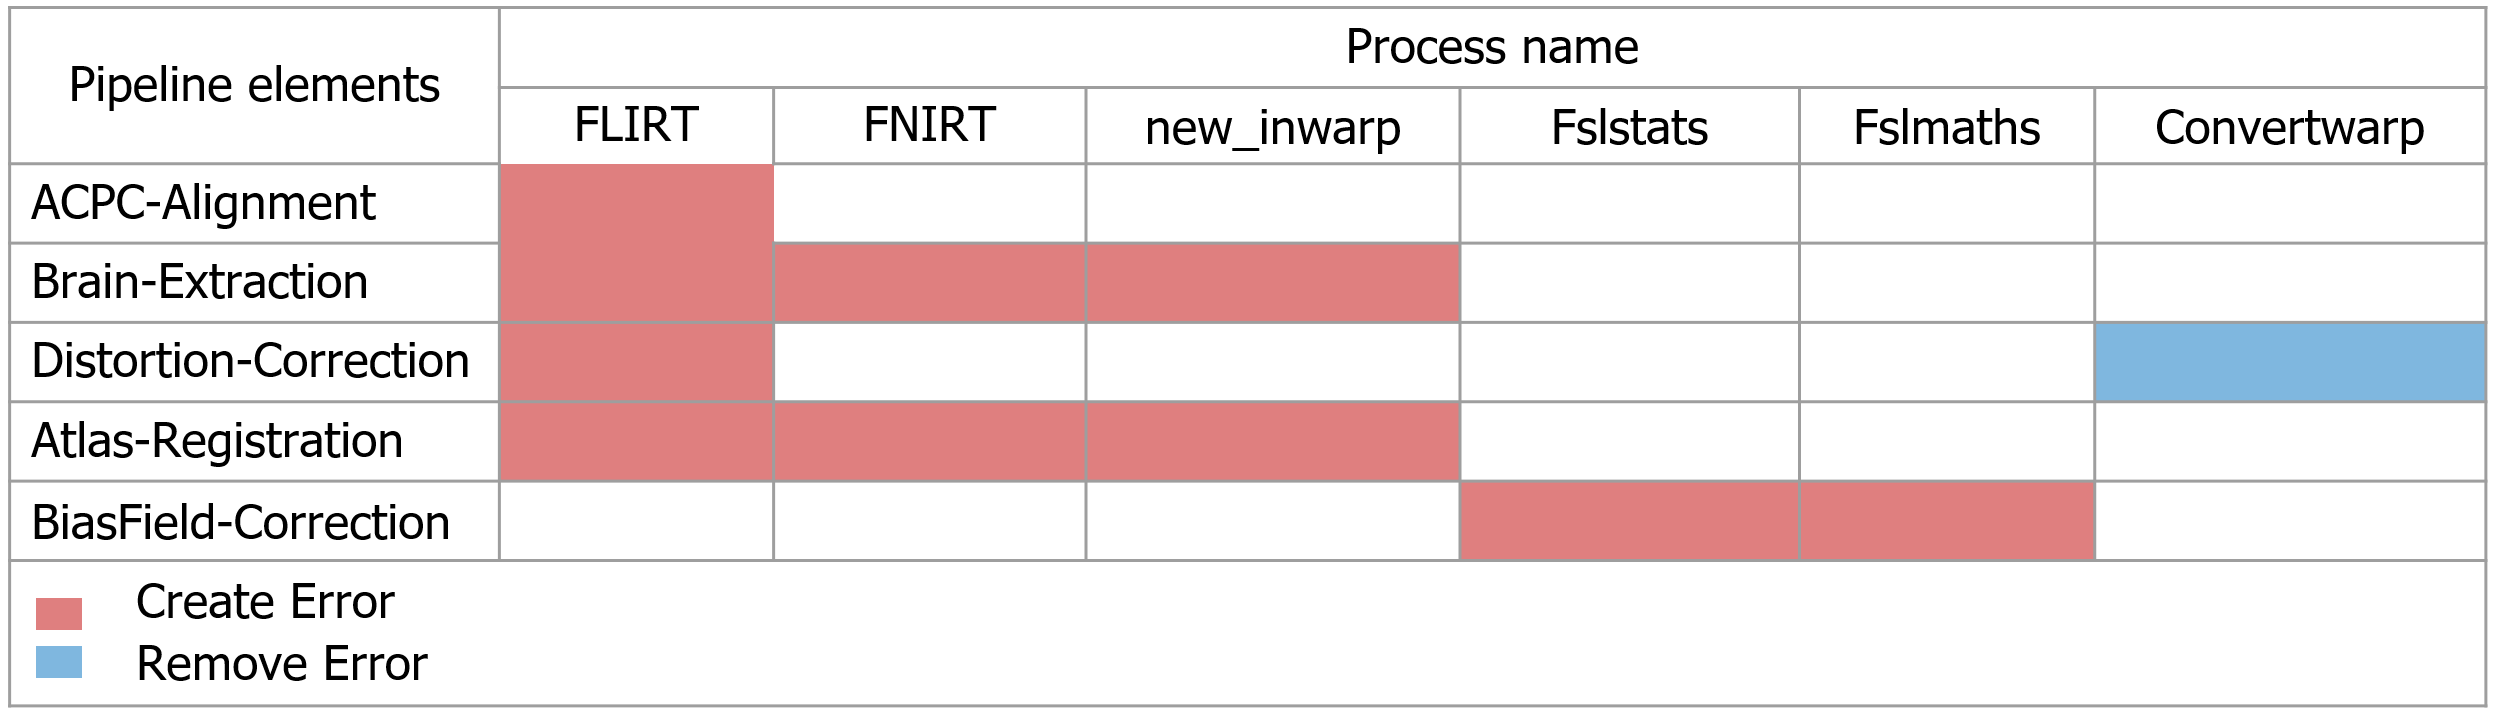
\includegraphics[width=\columnwidth]{images/pfs_table.png}
  \caption{Process name along with the pipeline elements that introduce 
  errors.}
  \label{fig:pfs_table}
\end{figure}

\begin{figure}
\centering
  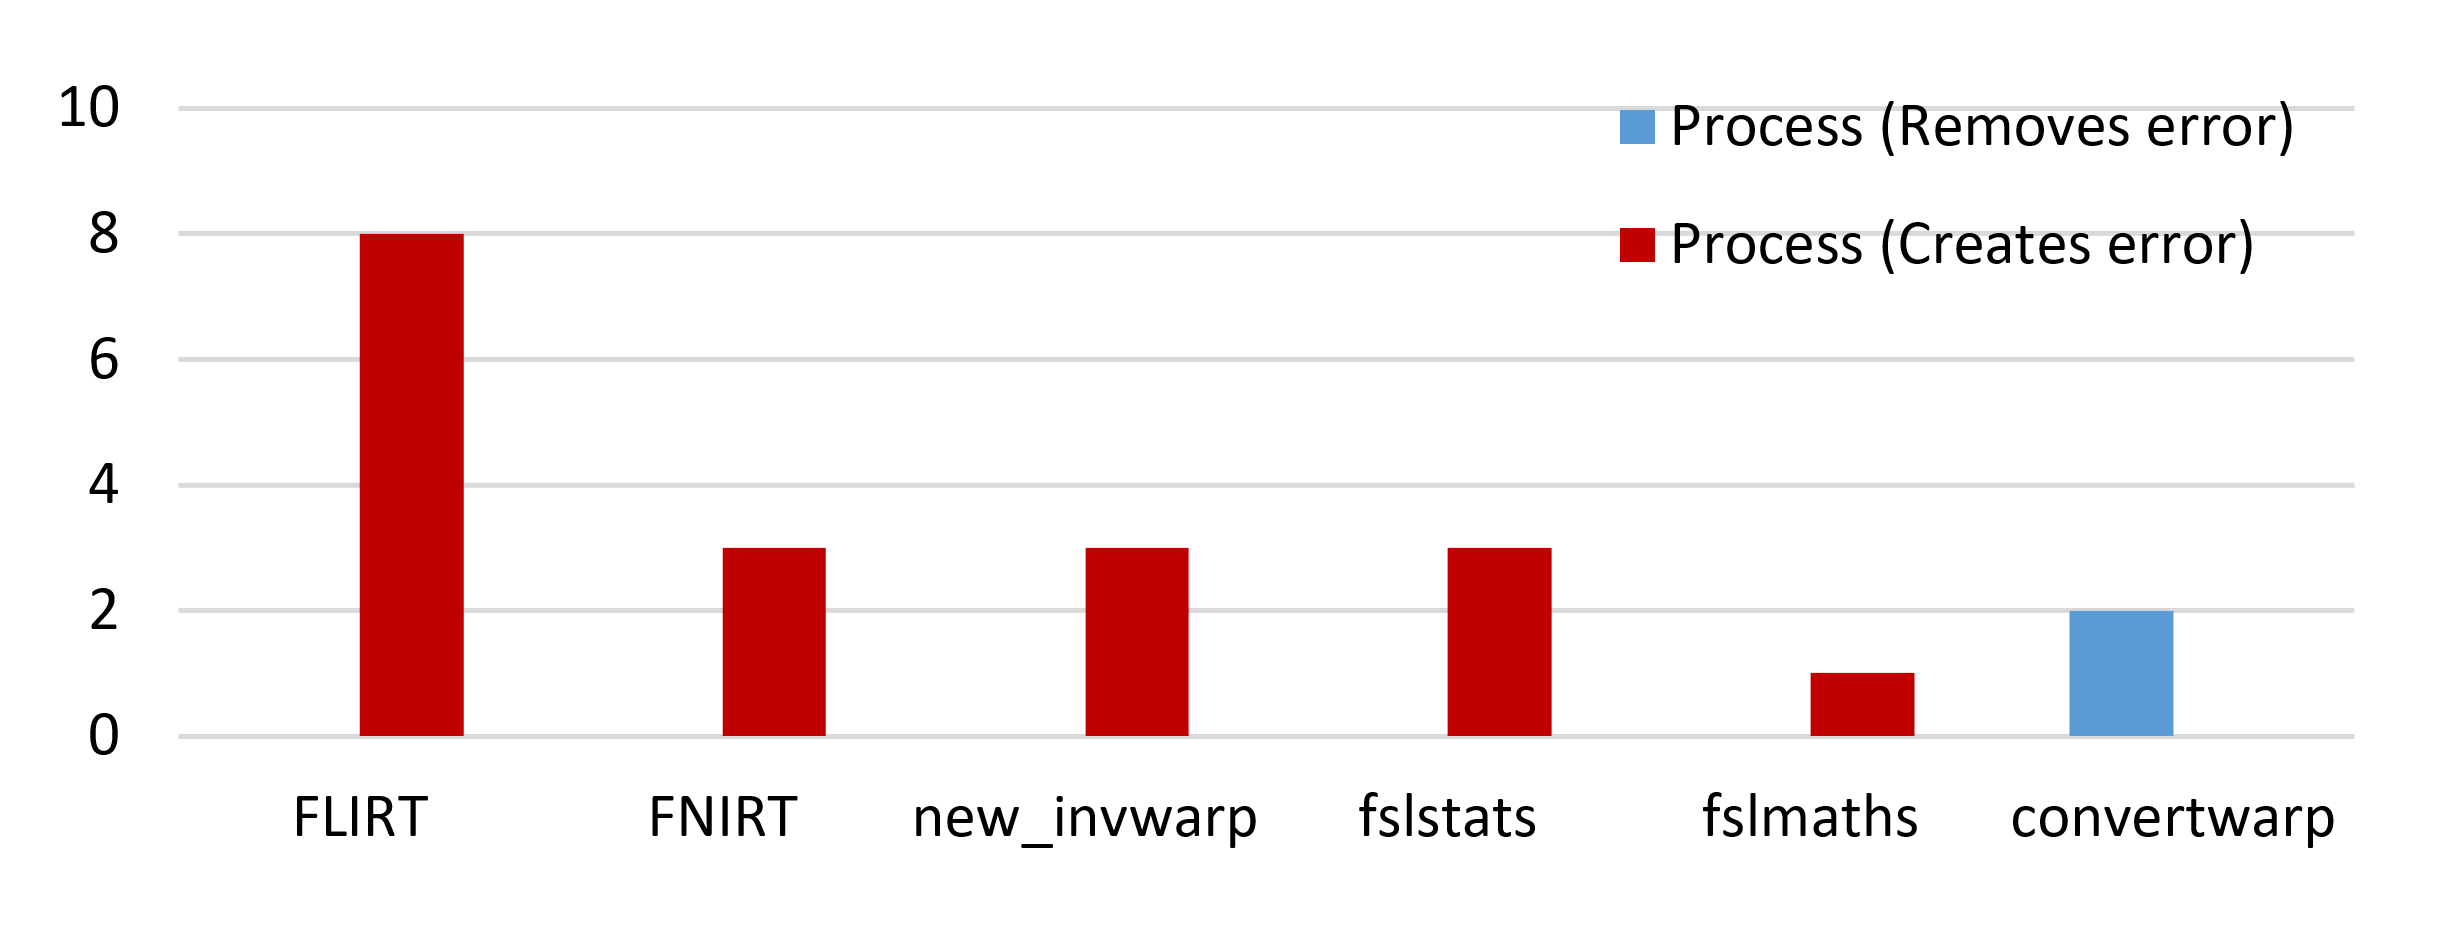
\includegraphics[width=\columnwidth]{images/pfs_chart.png} \caption{Number 
  of occurrences of errors in PreFreeSurfer on subject 103515, red and 
  blue bars indicate the processes which create and remove errors 
  respectively.} 
  \label{fig:pfs_chart}
\end{figure}


\section{Discussion}

\note{Pipeline amplify small numerical differences because they are numerically 
unstable. Furthermore, math libraries evolve over time, leading to 
different numerical errors. we listed some of the irreproducibility 
causes of the pipelines as we mentioned in the previous section 
overally along with exact command arguments.

Mention that this was only possible because the unprocessed data was 
shared in the first place. DICOM to Nifti conversion was out of scope 
and may introduce other issues.}

\section{Conclusion}

\note{Our technique is able to characterize the stability of a pipeline's 
components automatically. The numerical instability in the 
PreFreesurfer HCP pipeline arises mainly from linear and non-linear 
registration processes implemented in FSL FLIRT and FNIRT. 

There are a few ways to impede such instabilities:
\begin{itemize}
\item Use a single operating system
\item Containerize pipelines
\item Increase numerical precision
\item Be stricter on truncation and rounding standards (IEEE 754)
\item Build static executable
\end{itemize}

The results still suffer from small perturbations literally because of 
the fact that pipeline are not numerically stable. The preferred 
solution is to detect and fix numerical instability of the pipeline 
instead of masking the problem. These processes need to be reviewed to 
understand and correct the cause of instabilities. }


\section{Acknowledgments}

Data were provided by the Human Connectome Project, WU-Minn 
Consortium (Principal Investigators: David Van Essen and Kamil Ugurbil; 
1U54MH091657) funded by the 16 NIH Institutes and Centers that support 
the NIH Blueprint for Neuroscience Research; and by the McDonnell 
Center for Systems Neuroscience at Washington University.

\note{CBRAIN team. Compute Canada(Calcul Quebec).}

\begin{figure*}
\centering
  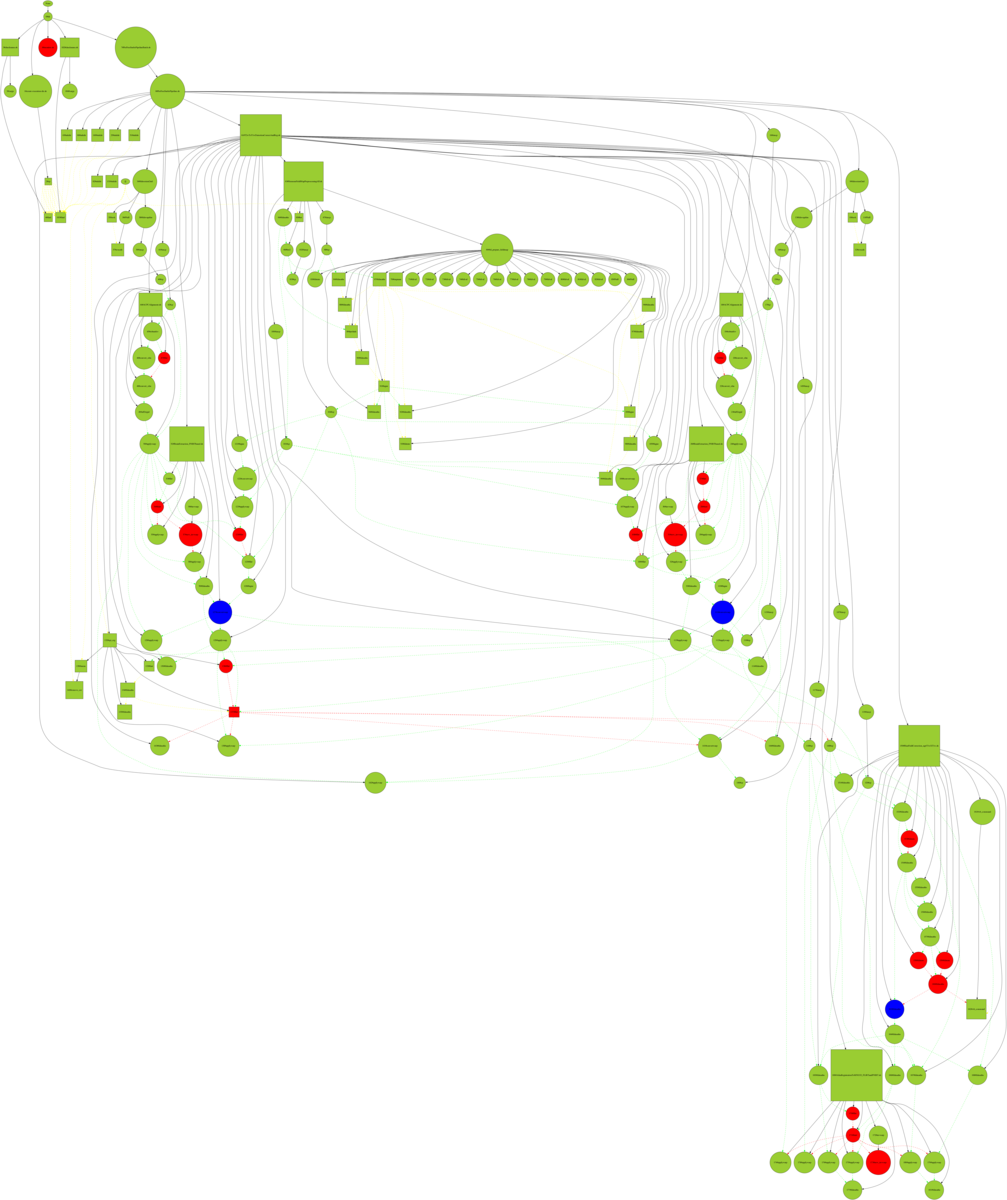
\includegraphics[width=.9\textwidth]{images/graph}
  \caption{A complete process graph from the PreFreesurfer pipeline.
Full-resolution image available at \url{https://drive.google.com/open?id=174yyn8SuVOUcK5aRVw0bagjDanLD0FLt}.}
  \label{fig:complete-graph}
\end{figure*}

\begin{figure*}
\centering
  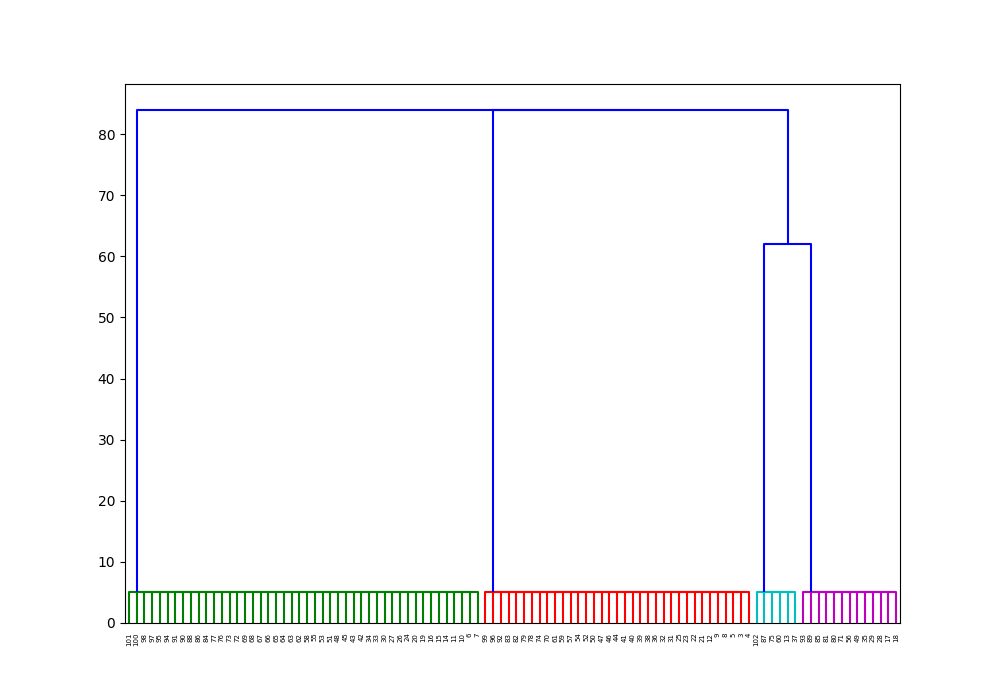
\includegraphics[width=.8\textwidth]{images/hclusters}
  \caption{Different data types clustered among 100 subjects.}
  \label{fig:subj-clusters}
\end{figure*}



\bibliographystyle{plain}
\bibliography{biblio}


\end{document}
